%###############################################################################
% LaTeX Presentation for Netizens
% Written by B[]
%
% -- Document Changes --
% Date       | Name     | Changes
% -----------|----------|-------------------------------------------------------
% 2016/04/06 | B[]      | Created document
%###############################################################################

%###############################################################################
% presentation.tex
%
% A presentation for reliable biometrics authentication for banking systems.
%###############################################################################

\documentclass{beamer}

\usepackage{listings} % Allows for code blocks to be used
\usepackage{textpos}  % Allows the logo to be inserted at a given position

% Defines the colours to be used in the presentation
\definecolor{secinhead}{RGB}{255,255,255}
\definecolor{titlebg}{RGB}{40,40,40}
\definecolor{frametitlefg}{RGB}{0,0,0}
\setbeamercolor{secsubsec}{fg=secinhead,bg=black}
\setbeamercolor{frametitle}{fg=secinhead,bg=titlebg}
\setbeamercolor{title}{fg=frametitlefg}
\setbeamercolor{titlelike}{fg=frametitlefg}

% Define the formatting for the code blocks
\lstset{
  backgroundcolor=\color{white},
  basicstyle=\ttfamily\scriptsize,
  breaklines=true,
  numbers=left,
  numbersep=5pt,
  numberstyle=\tiny\color{gray},
  rulecolor=\color{black},
}

% Define the headline layout
\setbeamertemplate{headline}
{
  \leavevmode
  \hbox
  {
    \begin{beamercolorbox}[wd=\paperwidth,ht=8.25ex,dp=3.5ex]{secsubsec}
      \raggedright
      \hspace*{2em}
      {\sffamily\Large\color{secinhead}\thesection.~\insertsection\hfill\insertsubsection}
      \hspace*{2em}
    \end{beamercolorbox}
  }
}

% Define the frame title page
\setbeamertemplate{frametitle}
{
  \vskip-3pt
  \leavevmode
  \hbox
  {
    \begin{beamercolorbox}[wd=\paperwidth,ht=1.8ex,dp=1ex]{frametitle}
      \raggedright\hspace*{2em}\small\insertframetitle
    \end{beamercolorbox}
  }
}

% Add the addition of the team logo
\addtobeamertemplate{frametitle}{}
{
  \begin{textblock*}{100mm}(.7\textwidth,-2.2cm)
    \includegraphics[height=1cm,width=1cm]{logo}
  \end{textblock*}
}

% Add information about the project in particular
\title[Crisis]{Reliable Biometrics for Digital Authentication}
\subtitle{Protecting Your Hard Earned Cash After Compromise}
\author{
  \includegraphics[height=2cm,width=2cm]{logo-black}
  \\
  Netizens
}
\institute{
  \inst{1}
  Cyber Security
  \\
  Computer Science
  \\
  University of Hertfordshire
}
\date{\texttt{\footnotesize April 2016}}

\begin{document}
  %#############################################################################
  % Introduction section
  %
  % Description: The first section of slides.
  %#############################################################################
  \section*{}
    %###########################################################################
    % Title frame
    %
    % Description: The first page the readers will see.
    %###########################################################################
    \frame{\titlepage}
  %#############################################################################
  % Introduction section
  %
  % Description: The first section of slides.
  %#############################################################################
  \section{Introduction}
    %###########################################################################
    % Contents frame
    %
    % Description: The contents page for all major future sections.
    %###########################################################################
    \subsection{Contents}
      \begin{frame}
        \frametitle{Contents}
        \tableofcontents[hideallsubsections]
      \end{frame}
    %###########################################################################
    % What will be covered
    %
    % Description: What will be covered in this presentation.
    %###########################################################################
    \subsection{Overview}
      \begin{frame}
        \frametitle{Overview}
        Considering authentication methods within the financial industry we look
        to propose how systems may be improved to better protect customers from
        fraudulent use. The proposed method uses \textbf{statistical data unique
        to the user} to increase the security of a connection.
      \end{frame}
    %###########################################################################
    % What the objectives are
    %
    % Description: What we aim to achieve with this presentation.
    %###########################################################################
    \subsection{Objectives}
      \begin{frame}
        \frametitle{Objectives}
        \begin{itemize}
          \item Current issues
          \item Generalise the problem
          \item Tackling the issue
          \item Future works
        \end{itemize}
      \end{frame}
  %#############################################################################
  % Current Issues section
  %
  % Description: Issues we are able to clearly demonstrate, but not very able
  %              to tackle.
  %#############################################################################
  \section{Current Issues}
    %###########################################################################
    % Demonstration of issues
    %
    % Description: Examples of the issues that exist.
    %###########################################################################
    \subsection{Quotes}
      \begin{frame}
        \frametitle{Bank Fraud}
        ``\emph{Thieves drain our bank accounts of more than £300 million pounds every year}" - BBC Watchdog, Online \cite{BBCFraud}
        \\
        \hfill
        \includegraphics[scale=0.25]{worried}\cite{WikiCommonsEmoji}
      \end{frame}
      \begin{frame}
        \frametitle{Bank Data}
        ``\emph{Globally, 22 data records were lost or stolen every second in 2015}" - Gemalto, Online \cite{Gemalto}
        \\
        \hfill
        \includegraphics[scale=0.25]{confused}\cite{WikiCommonsEmoji}
      \end{frame}
    \subsection{Examples}
      \begin{frame}
        \frametitle{Card, Chip \& Pin}
        \textbf{TODO:} Write this section.
      \end{frame}
      \begin{frame}
        \frametitle{Online}
        \textbf{TODO:} Write this section.
      \end{frame}
      \begin{frame}
        \frametitle{Others}
        \textbf{TODO:} Write this section.
      \end{frame}
  %#############################################################################
  % Generalisation section
  %
  % Description: Generalisation of the problem we are tackling.
  %#############################################################################
  \section{Generalisation}
    \subsection{Main Issue}
      \begin{frame}
        \frametitle{What is the issue here?}
        \textbf{TODO:} Write this section.
      \end{frame}
      \begin{frame}
        \frametitle{What does this mean?}
        \textbf{TODO:} Write this section.
      \end{frame}
  %#############################################################################
  % Tackling the issues section
  %
  % Description: Issues we are able to clearly demonstrate, but not very able to
  %              tackle.
  %#############################################################################
  \section{Tackling the Issues}
    \subsection{Reliability}
      \begin{frame}
        \frametitle{Main Algorithm}
        \textbf{TODO:} Write this section.
      \end{frame}
    \subsection{Hashes}
      \begin{frame}
        \frametitle{Card, Chip \& Pin}
        \textbf{TODO:} Write this section.
      \end{frame}
      \begin{frame}
        \frametitle{Fingerprints}
        \textbf{TODO:} Write this section.
      \end{frame}
      \begin{frame}
        \frametitle{Others}
        \textbf{TODO:} Write this section.
      \end{frame}
  %#############################################################################
  % Future Works section
  %
  % Description: Generalisation of the problem we are tackling.
  %#############################################################################
  \section{Future Work}
    \subsection{What Next?}
      \begin{frame}
        \frametitle{We need reliable hashes!}
        \textbf{TODO:} Write this section.
      \end{frame}
  %#############################################################################
  % Last section
  %
  % Description: The last section of slides, no breakdown is required in this
  %              section.
  %#############################################################################
  \section{Wrapping Up}
    %###########################################################################
    % Thanks frame
    %
    % Description: Thanking the listener to make them feel the warm and
    %              fuzzies.
    %###########################################################################
    \subsection{Thanks}
      \begin{frame}
        \frametitle{Thank You!}
        Any questions?
      \end{frame}
    %###########################################################################
    % References frame
    %
    % Description: The frame for the references.
    %###########################################################################
    \subsection{References}
      \begin{frame}[allowframebreaks]
        \frametitle{References}
        \begin{thebibliography}{3}
          \beamertemplateonlinebibitems
            \bibitem{WikiCommonsEmoji}
              Wiki Commons.
              \newblock {\em Emoji}.
              \newblock [Accessed 04-2016] Google - https://code.google.com/p/noto/,
              \newblock {\em Apache License 2.0: http://tinyurl.com/h8kzup7}
          \beamertemplateonlinebibitems
            \bibitem{BBCFraud}
              BBC Watchdog.
              \newblock {\em Bank Fraud: Easy to be a victim - hard to get your money back?}.
              \newblock [Accessed 04-2016] http://tinyurl.com/glrbl9k.
          \beamertemplateonlinebibitems
            \bibitem{Gemalto}
              Gemalto.
              \newblock {\em 2016 The Year Data Breaches Got Personal}.
              \newblock [Accessed 04-2016] http://tinyurl.com/h7vduvk.
        \end{thebibliography}
      \end{frame}
\end{document}
